\documentclass{bioinfo}
\copyrightyear{2005}
\pubyear{2005}

\usepackage[hyphens]{url}

\begin{document}
\firstpage{1}


\newcommand{\OnePhaseone}{phase1\_chr1}
\newcommand{\NinteenPhaseone}{phase1\_chr19}
\newcommand{\SevenPhaseone}{phase1\_chr1-7}
\newcommand{\FullPhaseone}{phase1\_chr1-22}
\newcommand{\OnePhasethree}{phase3\_chr1}
\newcommand{\ThreePhasethree}{phase3\_chr1-3}
\newcommand{\FullPhasethree}{phase3\_chr1-22}

\title[MapReduce Clustering]{Scalable Clustering of Genotype Information using MapReduce}
\author[O'Brien \textit{et~al}]{Aidan R O'Brien\,$^{1}$, Fabian A Buske\,$^{2}$ and Denis C. Bauer\,$^1$\footnote{to whom correspondence should be addressed}}
\address{$^{1}$CSIRO, Digital Productivity Flagship, 11 Julius Av, 2113, Sydney, Australia\\
$^{2}$Cancer Epigenetics Program, Cancer Research Division, Kinghorn Cancer Centre, Garvan Institute of Medical Research, 384 Victoria St, 2010, Sydney, Australia}

\history{Received on XXXXX; revised on XXXXX; accepted on XXXXX}

\editor{Associate Editor: XXXXXXX}

\maketitle

\begin{abstract}

\section{Motivation:}
Processing genomic information from whole genome sequence studies pose computational challenges due to the unprecedented data volume generated, which render transitional approaches insufficient. However, by utilising advancements in modern hardware accelerators and data processing we can provide the means for scalable solutions. We therefore aim to provide the interface between standard genomic data formats and advanced and scalable analysis libraries like Mahout. 
\section{Results:}
We achieve an 2-fold speedup by using the scalable k-means MapReduce implementation over the equivalent analysis performed in R, by comparable accuracy. However, the real benefit lies in scaling beyond R's capability to a population-size analysis. We successfully clustered more than 2,500 individuals each having more than 19 Million variants. 

\section{Availability:}
Using modern compute paradigms is essential to scale to modern genomic research in an efficient sustainable way. 

\section{Contact:} \href{Denis.Bauer@CSIRO.au}{Denis.Bauer@CSIRO.au}
\end{abstract}

\section{Introduction}

Grouping individuals based on the genomic profile is a commonly performed tasks to identify population structure~\cite{Gao2007} or elucidate different haplotype involvement in diseases susceptibility~\cite{Laitman2013}.  Traditionally both the number of individuals and included genotypes, typically from SNP arrays, were relatively small and libraries in Bioconductor sufficient. However, recent technological advances in whole genome sequencing have made population-scale sequencing feasible. It is hence economical to generate studies with sample sizes currently reserved for larger consortia such as the 1000 genomes project~\cite{1KG2012} or the cancer genome atlas (TCGA)~\cite{TCGA2013}. At the same time, whole genome sequencing enables the inclusion of rare or even somatic mutations in the analysis, increasing the feature space by orders of magnitude. This drastic increase in both sample numbers and features per sample requires a massively parallel approach to data processing. 

As a result of these big data challenges, MapReduce approaches are increasingly being used in bioinformatics (for reviews see~\cite{Zou2013, Qiu2010,Taylor2010}). This is especially the case for sequence analysis tasks, such as read mapping~\cite{Schatz2009}, duplicate removal~\cite{Jourdren2012}, and variant calling~\cite{Langmead2009, McKenna2010} as well as Genome Wide Analysis Study based tasks~\cite{Huang2013, Guo2014}.

%Mention Goolge's population clustering in the intro

At the same time, theoretical computer scientists adapt MapReduce paradigms to cope with the iterative nature of machine learning tasks~\cite{Chu2009}. Specifically, the Mahout project \url{https://mahout.apache.org/} has been developed extensively~\cite{Ranger2007, Owen2011} and was successfully applied in the clinical informatics space~\cite{Dong2013}.

In this paper we link the two areas of parallel machine learning and bioinformatics by providing an interface between Mahout and the standard variant data format, variant call format (VCF)~\cite{1KG2012}, which opens up the application of Mahout's different machine learning algorithms to be applied to genotype-based tasks. 

To demonstrate the capability we cluster variant datasets from the 1000 genomes project to determine population structure using the k-means clustering algorithm available in Mahout. In the first section we benchmark the performance and accuracy of Mahout's implementations against a standard R based implementation on a reduced version of the data and in the last two sections we investigate how Mahout scales to either more samples or more features per samples.   

%SeqWare~{OConnor2010} Libraries \cite{Doering2008,Schumacher2014,Nordberg2013}


\section*{Results and discussion}

% COMPARISON TO R
\subsection*{Clustering in Mahout requires less memory than in R}
In this section, we compare the runtime and resource requirements between the k-means clustering implementation in R and Mahout for the small \NinteenPhaseone{} dataset (see Methods). 
We measured the runtime separately for pre-processing stage as well as the clustering stage. 
%DB: can you explain 'container' or refer to methods where you have more room for discussing
With Hadoop, pre-processing the data takes approximately 6 minutes, with an allocation of up to 3GB memory per 'container'. The resulting data is stored as a Hadoop 'SequenceFile' of about 835MB in size.
Conversely,  pre-processing the data to R's in-memory matrix takes 56 minutes and required 17.7GB memory. 
K-means clustering the data, however, is faster with R, using 7s, whereas Mahout takes just under 9 minutes. See Table~\ref{Tab:02}. \\
Due to the relatively small number of variants, cluster performance is relatively poor for both methods, with the best Adjusted Rand Index score for clustering individuals in one of 4 populations (see Methods) being 0.705 in Mahout and 0.614 in R (see Table~\ref{Tab:02}).

Although the overall Mahout pipeline is about 40 minutes faster than R's, the actual k-means clustering takes two orders of magnitude longer in Mahout. 
This is due to the additional overhead involved in spawning the map and reduce processes, and distributing the data between nodes.
R, on the other hand, already has the entire matrix in-memory, on a single machine. 
Since no disk-access or networking is required the clustering can be performed faster. However, the amount of memory available on a single machine will quickly become a limiting factor. 
As an example, the entire set of 1000 Genome Project phase3 variants could require approximately 1.6TB to be completely loaded into memory as a double-precision matrix (see Table~\ref{Tab:01}). This is based on the equation:
$\frac{n \times m \times 8\text{bytes}}{1\text{GB}}$, where $n \times m$ are the matrix dimensions, 8bytes is the memory a double occupies (i.e. each matrix element), and  1GB is $10^9$bytes.

% DB: not clear you need to spell out your argument a bit more...
% AO: Fixed maybe
% DB: good explanation but I'm not sure what it does here (maybe reuse above or in methods)

%The primary benefit of Hadoop is its scalability. This is achieved through MapReduce jobs, which allow the task at hand to be separated into 'containers'.
%Although in the previous example, Hadoop had access to 36GB of memory distributed over 3 machines, the size of each container was only 3GB.
%Each of these containers is effectively a self-contained job that is independent from any other container.
%Therefore, the more resources that the user has available, the more containers that can be run in parallel, either on the same machine or separate, and in turn decreasing the run-time of the overall job.
%This means that our Hadoop job can scale from a single machine with minimal resources (albeit with a longer run-time), to a huge compute cluster with terabytes of RAM.
%This benefit allows Hadoop jobs to not only scale vertically, i.e. to a larger single machine as R can, but also horizontally, to a cluster of many machines.

% SCALING UP FEATURES IN MAHOUT
\subsection*{Hadoop scales to genome-wide clustering}
%DB phase 1 or phase 3 ?

In this section we demonstrate Mahout's scaling ability by increasing the number of features (variants per sample) to include the 38 million variants from the phase1 dataset (\FullPhaseone{}) and the 79 Million variants from the phase3 dataset (\FullPhasethree{}). 

We also ran jobs using intermediately sized phase1 datasets (see Table~\ref{Tab:02}) to demonstrate the different container sizes required by pre-processing and k-means clustering, and time required.
On the \OnePhaseone{} dataset, pre-processing takes just under 10 minutes and clustering takes approximately 12 minutes with the same container size as with the \NinteenPhaseone{} dataset.
We then increased the input to include the first seven chromosomes (\SevenPhaseone{}). In this case, pre-processing time increased to approximately 45 minutes, and clustering to 3 hours and 28 minutes.
Our pre-processing algorithm was successful with the same container size as the previous examples. However, we increased both the map and reduce container size for the clustering step to 4GB to accommodate the increased vector size.

Finally we used the entire phase one dataset as input. Although pre-processing now takes 85 minutes, it was again successful with the same sized containers as previously.
Clustering, however, not only required larger containers, but also took over 7 hours to complete.
%DB: you cannot use 'significant' without having performed some sort of statistical test to put a p-value to that statement. So use 'substantial' instead. Also this is a limitation from the cluster not a general thing so write it that way.

This substantial time increase is in part due to the larger container size. With each container allocated 6GB of memory, our cluster can only run up to six containers simultaneously, as opposed to 24 1.5GB containers (from the smaller examples).
This restriction in simultaneous containers is due to the limited memory available on our cluster.

Although we compare phase3 datasets in the next section because they have a larger number of samples, the \FullPhasethree{} dataset also has the largest feature size, so we mention that in this section to demonstrate Hadoops ability to scale with feature-size.
The most notable difference is the time required to complete clustering, at just over 21 hours. Although this is a substantial increase in time, the job still completes successfully. As we mention in a later section, this time can be reduced dramatically on a larger cluster.
% DB: we need to discuss why the accuracy is actually dropping when you include more chromosomes. Its counterintuitive ... do you have a suggestion?

%While R does not scale to the larger datasets datasets, we have demonstrated Hadoop to cope well with pre-processing and clustering variants from 22 phase1 VCF files.
This section demonstrates Hadoop's ability to cope with genome wide information, which predominately inures a runtime increase. Although a memory increase is also present, the memory increases in proportion to vector length, rather than the size of the dataset, meaning we could still successfully run a job
on the variants from an entire genome without encountering limitations due to the memory our cluster has available.
%rather than memory increase which quickly become the limiting factor as demonstrated by R's inability to process the data. 

% SCALING UP SAMPLES IN MAHOUT
\subsection*{Hadoop scales effortlessly to more than twice the number of samples}
% Can you rewrite this section to lead to the below concluding statement
In this section we investigate Mahout's ability to scale with more samples, i.e. the 2504 individuals from the phase3 dataset compared to the 1092 individuals in the phase1 dataset. We focus on the \SevenPhaseone{} and \ThreePhasethree{} datasets due to their relatively similar feature size.

The container size required for pre-processing the data is identical for both datasets, however the \ThreePhasethree{} dataset requiring about twenty minutes more time than the smaller \SevenPhaseone{} dataset.
The clustering accuracy is 0.813 for the phase1 dataset and 0.825 for the phase3 dataset.
%In this case, due to the number of Feature Vectors increasing, rather than the feature size, we expect the memory requirements for k-means clustering should remain similar, as the cluster centres loaded into the containers' memory are approximately the same size.
%We expect the memory requirement for the k-means clustering to stay the same as the number of cluster centres loaded into the containers' memory remain constant despite the increase of feature vectors oppose to feature size.
We expect the memory requirement for the k-means clustering algorithm to be the similar for both datasets, because the larger size of \SevenPhaseone{} is due of more feature vectors (more individuals), rather than larger feature vectors (more variants).
Mahouts iterative k-means algorithm loads a set number of these vectors into memory, based on the number of k-means clusters. And therefore, if the feature size doesn't increase, this memory requirement also won't increase.
This proved to be the case, as 4GB allocated per container was the minimum for both datasets.

%DB: do you agree with this concluding statement?
%Scaling effortless to massively more samples is the strength of Hadoop, hence compute problems need to be carefully designed to harness this ability.  
%Hadoop's strength is billed to be its ability to scale to massively more samples, however on a finite-resource cluster we observe a limitation to this scalability, which results in a dramatic increase in runtime. 
Hadoop's strength is billed to be its ability to scale to massively more samples. We observe this to be true, as increasing the samples by more than twice, which is the case from \SevenPhaseone{} to \ThreePhasethree{}, does not result in greater memory requirements, unlike increasing the number of variants per sample.

\subsection*{Result visualisation }
% DB: in the conclusion we discussed that we provide a "toolset to interpret Mahout's clustering output". We hence need to show the R-image for that, i.e. spit out distance matrix and read in with R to plot, e.g. doing Multidimensional Scaling to squash the matrix in 2D http://www.statmethods.net/advstats/mds.html 

% AO: new section
\subsection*{Cluster size and containers}
An important consideration when designing a MapReduce job is the container size. A container is essentially an abstraction of resources, i.e. memory and CPU cores. Tasks are run in parallel in these containers, and each container is independent of other containers.
The resources Hadoop allocates to each container is a predefined value, specified in its configuration. According to the Cloudera documentation, the general rule of thumb is that one CPU core is allocated to each container, and the available memory per node should be divided equally between each of those containers. For example, on a node with 8 CPU cores and 32GB memory, each container should be allocated 1 CPU core and 4GB Memory. Effectively allowing a maximum of eight 4GB containers to run in parallel on that node.

When a MapReduce job is launched, Hadoop spawns a number of map tasks and reduce tasks. These tasks are placed in a queue until a node has resources available to run a container.
The more containers that can run simultaneously, the faster the job will complete. Generally, the number of containers is limited by the available CPU cores, as each container requires an entire CPU core. However for jobs that deal
with large datasets, the memory allocated per container may not be enough.
We could modify the above example to allocate each container 1 CPU core and 8GB memory, however now only four containers can fit within the node's 32GB memory, resulting in the other 4 CPU cores being disused. It is therefore optimal to
allocate the appropriate resources to containers, and only increase container memory when necessary, as overallocation of memory will simply limit the number of simultaneous containers each node can run.

To demonstrate the importance of specifying these parameters correctly, we ran the same job using different configurations. The relatively small job, \OnePhaseone{}, took an additional 5 minutes with a map container size of 4GB, as opposed to 1.5GB.
Yet this larger container size is still too small for the \FullPhasethree{} dataset, which requires at least 6GB allocated to each map container.

To demonstrate the scaling ability of jobs to a larger cluster, we ran the same clustering job on a development cluster we had access to. As presented in Table \ref{Tab:03}, the \OnePhaseone{} job saw an improvement of approximately 70\%.
The \FullPhasethree{} example, on the other hand, was 78\% faster.
A limitation in both these examples is that the number of reduces in k-means clustering is limited to the number of k-means clusters. A task with five clusters, for example, will only be able to spawn five reduce containers, no matter how many resources are available.






\section*{Conclusion}
In this paper we have applied Mahout's k-means clustering to the task of clustering individuals, based on their genomic variants. 
We provide an interface from VCF format to Hadoop and Mahout, and a toolset to interpret Mahout's clustering output (see Figure 1)
We find that on small datasets the clustering stage is two orders of magnitudes slower in Mahout compared to R (9 minutes vs 7 seconds), due to the overhead of setting up and co-ordinating the communication between the Hadoop nodes. 
However, increasing either the number of samples or the number of features per sample quickly exceeds the capability of R on this machine due to memory limitations.
%DB ok effortlessly might be overstated ?
Hadoop on the other hand scales effortlessly to more than twice the number samples (2,504) and can process VCF files that contain over 79 Million variants per samples.
The MapReduce functions can scale from a relatively small and accessible cluster with 16 cores, to a much larger cluster with close to 500 CPU cores. 
In conclusion, Mahout offers a scalable out-of-the box solution that is directly applicable to genotype-based clustering for population or family association. 

%This efficient a high performance in-memory map-reduce system has already demonstrated to deliver a  50x speed-up on a whole-genome dataset compared to usual multithreaded approaches, see ADAM~\cite{Massie2013}


\begin{methods}
\section{Methods}
\subsection*{Datasets}
We used variant call format (VCF) files from phases 1 and 3 of the 1000 Genomes Project.
Each VCF file details the genetic variation (SNPs and indels) for one chromosome, between each individual and a reference genome derived from GRCh37. 
The phase1 and phase3 datasets contain 1,092 and 2,504 individuals, respectively.
Metadata available from the 1000 Genomes Consortium specifies additional attributes for each individual, including population and familial data.\\
We used different subsets of the data for different comparisons. For example, to be able to compare Hadoop with R, we used the VCF file containing chromosome 19 variants (\NinteenPhaseone{}).
To demonstrate scaling with Hadoop, we use subsets that contain more variants, i.e. \SevenPhaseone{} and \FullPhaseone{}, which include chromosome 1-7 and the full genome, respectively.
Table~\ref{datasets} contains an overview of the datasets.

\subsection*{Hardware and Software}
%DB what about Piotr's cluster I thought you used that one for the full genome data of phase 1 and phase 3 ?
We processed the data using a cluster of five VMs on the Microsoft Azure cloud service. Three of these VMs, the 'worker nodes', each have 14GB memory and and 8 CPU cores. These three VMs run the Hadoop2 NodeManager, which manages the Yet Another Resource Negotiator (YARN) 'containers'.
The user is able to specify the resources allocated to each container, where map containers can have a different allocation to reduce containers.
The fourth VM runs the HDFS NameNode, ResourceManager and monitoring services, and the fifth VM, a small, single core machine, runs the Cloudera manager service.
With a total of 42GB memory and 24 CPU cores available between the node managers, we can simultaneously run up to 24 YARN containers with 1.5GB memory per container, or 12 YARN containers with 3GB memory per container.
Storage consists of a 3TB Hadoop Distributed File System (HDFS) partition distributed across the three worker nodes. Each of these nodes runs a DataNode with a 1TB disk.

We used a single VM for the comparison between Mahout and R.

\subsection*{Pre-processing}
\label{Sec:preprocessing}
Mahout requires Hadoop's `SequenceFiles' as input to its machine learning algorithms. SequenceFiles are binary flat files consisting of key/value pairs. In this case, each of the keys is a
label for an individual, where the associated value for each key is a `sparse vector' representing the individual's genomic variants. We use sparse vectors, rather than
dense vectors, to significantly reduce required memory and disk space. Each sparse vector consists of two separate vectors. An item in the first vector is
effectively a key for an item at the same position in the second vector. The key represents a genomic location, where its value represents the variant. Zero values (positions where there is no variant)
are omitted. Therefore, the fewer variants in an individual's genome, the smaller the sparse vector size. In comparison, `dense vectors' are single arrays that
include every position where a variant may fall, whether or not there actually is a variant. Therefore, the size of a dense vector isn't reduced with a large number of non-variants.

The values of the sparse vectors, which, as previously mentioned, represent an individuals genomic variants, are a \texttt{double} java type.
We set the value of each double to the sum of the square root of the Hamming distance between each variant allele and the reference genome. Therefore, a value identical to the reference, 0\textbar{}0, will be 0 (and omitted from the sparse vector),
a heterozygous variant, 0\textbar{}1 or 1\textbar{}0, will be 1 (sqrt1) and a homozygous variant, 1\textbar{}1, will be 2 (sqrt1 + sqrt1). The square root of the each allele prevents variants such as 1\textbar{}1 colliding with the variant 2\textbar{}0.

We wrote two `MapReduce' classes in Java to convert VCF files to the aforementioned sequence files. This is scalable and should work on any number of files,
of any file size; limited only by disk space and time. 
The `map' stage of the first job parses each line of the VCF file to key value pairs. Each of the keys are an identical arbitrary number, where the value for each key is a sparse vector of the variants from each line. The variants in each vector are in the same order as they appear in the VCF file.

Additionally, in this stage, we can define parameters to exclude certain variants that may be deemed low quality, or only appear in a certain number of individuals.
We use identical keys so that each key value pair is sent to the same reducer, and this reducer assigns a unique key to each value. We require one reducer in this step to make each the key for each variant a consecutive number, rather than an arbitrary feature, such as its genomic location. Because keys are represented by integers, this helps to avoid integer overflows by keeping the keys relatively small.

The second job effectively transposes the output from the first job. The mappers create key value pairs where the key is a composite of the individual id and variant id, and the value is the variant.
This composite key, which is essentially a concatenation of two keys, allowed us to implement custom 'collect' and 'sort' classes to speed up the process. These classes divide up the key value pairs by their individual ID and sort them by their location ID, so each sorted collection of key/value pairs can be sent to a separate reducer.
 The reducers then write the variants for each individual to a sparse vector and stores each vector as a value, where the key is the individual ID.


\subsection*{Mahout K-means clustering}
To cluster the samples from the sequence files, we use Mahout 0.9 with Hadoop 2.5.0. 
The clustering steps are the same for each dataset, however, due to the increased feature size we designate more memory to the
YARN containers. For the first step, we specify \texttt{k}, the number of clusters. The function \texttt{RandomSeedGenerator.buildRandom} creates a new sequence file containing \texttt{k}
random centroids from the samples sequence file. The sequence file
of samples and the sequence file of centroids serve as the input to \texttt{KMeansDriver.run}, a static Mahout API function that launches
a k-means clustering job on the Hadoop service. 


\subsection*{R K-means clustering}
We use `readVcf' from the R library, `VariantAnnotation', to iteratively read in the VCF file. For each iteration, we convert the data to a matrix and
convert the values for each variant to a double, as mentioned previously. We then transpose the matrix, so individuals are represented
by rows, and append the matrix to that from the previous iteration. Once the matrix contains all of the variants from the VCF file, we cluster the data
using the `kmeans' algorithm from the `stats' library.



\subsection*{Clustering quality}
We scored the clusters with the Adjusted Rand index~\cite{Hubert1985}. 
This index compares two different cluster sets, here the prediction $X = \{ X_1, X_2, \ldots , X_r \}$ and the annotated data $Y = \{ Y_1, Y_2, \ldots , Y_s \}$, and assigns a value based the overlap between $X$ and $Y$ as captured in a contingency table $\left[n_{ij}\right]$ where each entry $n_{ij}$ denotes the number of objects in common between $X_i$ and $Y_j : n_{ij}=|X_i \cap Y_j|$. 
The Adjusted Rand index is then 
{\tiny
\begin{eqnarray*}
ARI=\frac{\sum_{ij}{{n_{ij}\choose 2}} - \left[ \sum_{i}{{a_i\choose2}} \sum_{j}{{b_i\choose2}} \right] / {n\choose2}}{\frac{1}{2} \left[ \sum_{i}{{a_{i}\choose 2} + \sum_{j}{{b_{j}\choose 2}}} \right] - \left[ \sum_{i}{{a_{i}\choose 2} + \sum_{j}{{b_{j}\choose 2}}} \right] / {n\choose2}} 
\end{eqnarray*}
}
where $a$ and $b$ are the sums over the rows and columns of the contingency table.

The value is zero for independent clusterings and one for identical clusterings. 
We compared the Mahout k-means clusters and the R k-means clusters to the known clusters based on meta data from the 1000 genome project.
For the known clusters, individuals from the both phase1 and phase3 datasets were partitioned by their super population code, ASN, EUR, AFR, and AMR, where phase3 included EAS and SAS instead of ASN.



\subsection*{Performance}
We recorded the job time from the 'Elapsed' time as reported by the Hadoop JobHistory server. This is measured from the job's start time to finish time.
Because k-means clustering performs multiple iterations, and therefore spawns multiple MapReduce jobs, the time we reported is the sum of the elapsed time of each job.
For the R job, where we could not easily separate the pre-processing and clustering components, we printed the time between
stages using the function, \texttt{proc.time()}.

\end{methods}

\begin{table}[!t]
\processtable{Datasets used in this study.\label{Tab:01}}
{\begin{tabular}{lrrrrr}\toprule
name& individuals & variants & in-memory  & population\\
& & &size (GB) &groups& \\\midrule
        \NinteenPhaseone{} & 1,092 & 816,115 & 7.13  & 4\\
        \OnePhaseone{} & 1,092 & 3,007,196 & 26.27  & 4\\
        \SevenPhaseone{} & 1,092 & 18,984,880 & 165.85 & 4\\
        \FullPhaseone{} & 1,092 & 38,219,238 & 333.88 & 4\\
	\OnePhasethree{} & 2,504 & 6,468,094 & 131.17 & 5\\
	\ThreePhasethree{} & 2,504 & 19,381,970 & 393.06 & 5\\
	\FullPhasethree{} & 2,504 & 79,000,000 & 1602.00 & 5\\\botrule
\end{tabular}}{Datasets used in this study; based on portions of the phase1 and phase3 data from the 1000 genomes project.
In-memory size is the approximate memory required to store the data as a double-precision matrix of size n,m using the formula: n*m*8bytes/10\textsuperscript{9}bytes.
}
\end{table}

\begin{table*}[!t]
\processtable{Resources allocated and time taken.\label{Tab:02}}
{\begin{tabular}{ll|cc|cc|rr|c}\toprule
Tool & Dataset & \multicolumn{2}{ c |}{Preprocesing (GB)} & \multicolumn{2}{ c |}{Clustering (GB)} & \multicolumn{2}{ c |}{Time} & Accuracy\\
& & map & reduce  & map & reduce  & pre-processing & clustering & \\\midrule
        R &\NinteenPhaseone{} & - & - & - & - & 55m 41s & 7s &0.614\\
        Mahout & \NinteenPhaseone{} & 1536 & 3072 & 1536 & 3072 & 6m 10s & 8m 32s & 0.705\\
        & \OnePhaseone{} & 1536 & 3072 & 1536 & 3072 & 9m 52s & 12m 49s & 0.798\\
        & \SevenPhaseone{} & 1536 & 3072 & 4096 & 4096  & 43m 56s & 3h 28m & 0.813\\
        & \FullPhaseone{} & 1536 & 3072 & 6144 & 6144  & 85m 29s & 7h 43m & 0.723\\
        & \OnePhasethree{} & 1536 & 3072 & 1536 & 3072 & 23m 27s & 21m 14s & 0.622\\
        & \ThreePhasethree{} & 1536 & 3072 & 4096 & 4096 & 63m 49s & 4h 21m & 0.825\\
        & \FullPhasethree{} & 1536 & 3072 & 6144 & 6144 & 5h 36m & 21h 5m &0.840\\\botrule
\end{tabular}}{The resources allocated to each MapReduce yarn-container and time taken for the job(s) to complete.}
\end{table*}


\begin{table*}[!t]
\processtable{Resources allocated and time taken.\label{Tab:03}}
{\begin{tabular}{l|cc|cc|r}\toprule
Dataset & \multicolumn{2}{ c |}{Available Resources} & \multicolumn{2}{ c |}{Container Size (GB)} & Time\\
& CPU cores & Memory (GB)  & map & reduce & \\\midrule
        \OnePhaseone{} & 24 & 36 & 1536 & 3072 & 12m 49s\\
        \OnePhaseone{} & 24 & 36 & 4096 & 4096  & 17m 47s\\
        \OnePhaseone{} & 448 & 1310 & 1536 & 4096  & 5m 22s\\
        \FullPhasethree{} & 24 & 36 & 6144 & 6144 & 21h 4m\\
        \FullPhasethree{} & 448 & 1310 & 6144 & 6144 & 4h 42m\\\botrule
\end{tabular}}{The resources allocated to each MapReduce yarn-container and time taken for the job(s) to complete.}
\end{table*}


\begin{figure}[!tpb]%figure1
\centerline{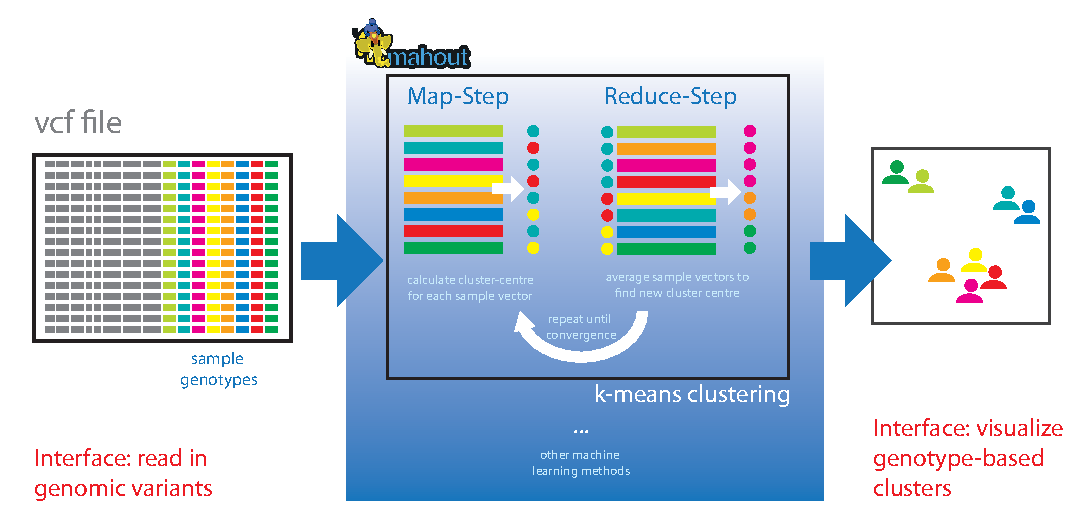
\includegraphics[type=pdf,ext=.pdf,read=.pdf, scale=0.40]{signature}}
        \label{fig:sign}
        \caption{{\bf Illustration of Mahout-based clustering of genotypes.}
      The image shows how the here introduced interface converts the VCF file to a mahout usable vector-based data type. Based on k-means it illustrates how the Map-step procedure groups of vectors by their nearest cluster center and the Reduce-step averages the vectors in each group to find the new value of the updated cluster center. The mahout-produced output is then converted into a visualisation.}

\end{figure}





\section*{Acknowledgement}
A.R.O was funded by the NSW Cancer Institute Big Data Big Impact schema, F.A.B by the National Health and Medical Research Council [1051757] and D.C.B by Commonwealth Scientific and Industrial Research Organisation's Transformational Capability Platform, Science and Industry Endowment Fund and Information Management and Technology Services.
The authors would like to thank Piotr Szul and Gareth Williams for their help with setting up Hadoop on the HPC system.  

\bibliographystyle{natbib}
%\bibliographystyle{achemnat}
%\bibliographystyle{plainnat}
%\bibliographystyle{abbrv}
%\bibliographystyle{bioinformatics}
\bibliography{genotypeClustering}  
\end{document}
